\section{Object Multiplex}

\label{app:multiplex}
As discussed in \S\ref{app:sec:limitations}, \model’s video pipeline performs memory processing independently per tracked object and uses minibatch parallelism for multi-object tracking. While this design is simple and effective, it leads to compute and memory costs that grow linearly with the number of objects and limits shared context in crowded scenes. To address this, we present SAM 3 \emph{Multiplex}, a shared-memory approach that enables joint multi-object processing within \model’s existing tracking pipeline.

\subsection{Formulation}
\begin{figure}[h]
	\centering
	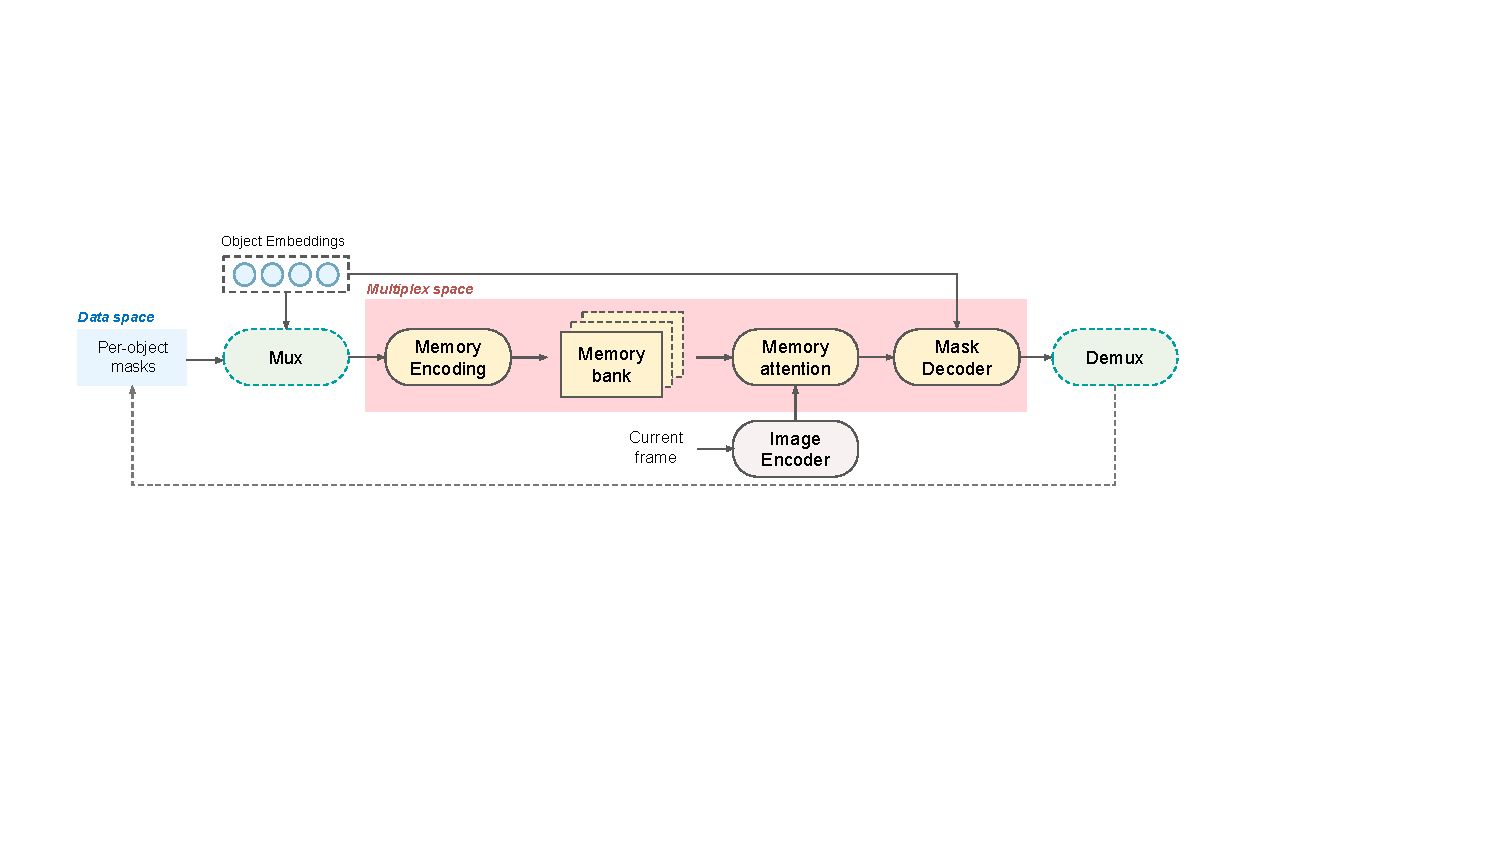
\includegraphics[width=\linewidth]
    {figures/h_multiplex/multiplex_diagram.pdf}
    \vspace{-15pt}
	\caption{\model Multiplex overview. Per-object masks are grouped via \emph{mux} into buckets for joint processing. Memory encoding, attention, and mask decoding operate in \emph{multiplex space}, with object embeddings preserving per-object identity. Bucket-wise outputs are unpacked via \emph{demux} to recover per-object masks in the \emph{data space}.}
	\label{fig:multiplex_diagram}
    \vspace{-5pt}
\end{figure}

\paragraph{Overview}
Inspired by data multiplexing networks~\citep{murahari2022datamux}, we reformulate \model's object-specific memory processing as a shared-memory computation that operates on multiple objects jointly. The key idea is to group objects into fixed-capacity \emph{buckets} with $M$ slots (we use $M{=}16$ by default), and to perform memory encoding and retrieval \emph{once per bucket} rather than once per object. This reduces the number of bucket-level memory-path  forward passes from $O(N)$ to $O(\lceil N/M \rceil)$. For example, with $M{=}16$, tracking 16 objects requires a single bucket pass instead of 16 separate passes.
This batched computation is effective in practice because per-object memory features are largely spatially disjoint in most frames; overlaps are sparse, so joint encoding preserves object-specific information while avoiding redundant computation.

Multiplex factorizes object information into (i) a \emph{shared spatial memory} and (ii) \emph{object-specific embeddings}. The shared spatial memory is produced by encoding the image features together with the bucket's (slot-wise) mask signals, yielding a single memory representation for all objects in the bucket. Object-specific embeddings preserve per-object identity throughout the pipeline: they are stored in the memory bank alongside spatial features for temporal association, and are provided to the mask decoder to ensure correct attribution of shared features to individual objects.
This design is conceptually aligned with prior video segmentation systems~\citep{AOT, DeAOT, AUSM} that combine shared representations with object identity cues, and can be viewed as adapting established multiplexing principles to \model while leaving the overall tracking pipeline unchanged.

\paragraph{Mux/Demux}
\Cref{fig:multiplex_diagram} illustrates the multiplexed memory pathway, including mux/demux operations. We define two complementary operators that convert tensors between (i) \emph{data space}, where tensors are indexed by object, and (ii) \emph{multiplex space}, where tensors are indexed by bucket and slot. \emph{Mux} maps per-object mask signals (and corresponding object-specific embeddings) into bucketed tensors according to a bucket-slot assignment, enabling bucket-wise execution of the memory pathway. \emph{Demux} performs the inverse mapping, unpacking slot-indexed outputs back to per-object predictions by reusing the recorded assignment. 

Following \model's multiple mask prediction approach designed to handle ambiguity, each slot produces three candidate masks, yielding $3M$ masks per bucket from which the best mask per object is selected. This does not significantly increase runtime, as the decoder outputs a fixed set of five tokens per slot (three mask tokens, one IoU token, and one object-score token), for a total of $5M$ tokens per bucket ($5 \times 16 = 80$ when $M{=}16$). During training, we randomize slot indices within each bucket to encourage permutation robustness.

\subsection{Results}
\paragraph{Video PCS with Text Prompt} 
We present \model Multiplex performance of video segmentation with text prompts on both our SA-Co/VEval benchmark and existing public benchmarks in \Cref{table:multiplex_vis}, following the evaluation protocol in \S\ref{app:video_grounding_details}. For fair comparison, \model Multiplex uses the same detector as SAM 3.
On SA-Co/VEval benchmark, \model Multiplex demonstrates improvements across all three test splits, with the most notable gains on YT-Temporal-1B ($+2.7$ cGF, $+0.9$ pHOTA), while on public benchmarks, results are mixed with improvements on OVIS ($+1.8$ mAP) but slight regressions on LVVIS, BURST, and YTVIS21. 

	\begin{table*}[hb]
		\vspace{5pt}
		\centering
		{
			\fontsize{\mytablesize}{\mytablebaselineskip}\selectfont
			\begin{tabular}{y{70}x{16}x{20}x{16}x{20}x{16}x{20}x{35}x{35}x{31}x{31}}
				& \multicolumn{6}{c}{\textbf{\evalvid benchmark test split}} & \multicolumn{4}{c}{\textbf{Public benchmarks}} \\
				\cmidrule(lr){2-7} \cmidrule(lr){8-11}
				& \multicolumn{2}{c}{\textbf{SA-V}} & \multicolumn{2}{c}{\textbf{YT-Temporal-1B}} & \multicolumn{2}{c}{\textbf{SmartGlasses}} & \textbf{LVVIS} & \textbf{BURST} & \textbf{YTVIS21} & \textbf{OVIS} \\
				& \multicolumn{2}{c}{(2.0K NPs)} & \multicolumn{2}{c}{(1.7K NPs)} & \multicolumn{2}{c}{(2.4K NPs)} & \hspace*{-2pt}(1.2K~NPs) & (482 NPs) & (40 NPs) & (25 NPs) \\
				\cmidrule(lr){2-3} \cmidrule(lr){4-5} \cmidrule(lr){6-7} \cmidrule(lr){8-8} \cmidrule(lr){9-9} \cmidrule(lr){10-10} \cmidrule(lr){11-11}
				\textbf{Model} & \hspace*{-2pt}\cgf & \hspace*{-4pt}pHOTA & \hspace*{-2pt}\cgf & \hspace*{-4pt}pHOTA  & \hspace*{-2pt}\cgf & \hspace*{-4pt}pHOTA  & test mAP & test~HOTA & val~mAP & val~mAP \\
				\midrule
				\textbf{\model} & 30.3 & 58.0 & 50.8 & 69.9 & 36.4 & 63.6 & \textbf{36.3} & \textbf{44.5} & \textbf{57.4} & 60.5 \\
                \textbf{SAM 3} Multiplex & \textbf{30.5} & 58.4 & \textbf{53.5} & \textbf{70.8} & \textbf{36.5} & \textbf{64.4} & 34.2 & 43.1 & 56.3 & \textbf{62.3}\\
                \textbf{SAM 3.1} Multiplex$^{\dagger}$ & \textbf{30.5} & \textbf{58.7} & 52.9 & 70.7 & 36.3 & \textbf{64.4} & 34.3 & 43.3 & 56.6 & 61.5\\
			\end{tabular}
            \vspace{-10pt}
        \caption{\small Video PCS results comparing \model and \model Multiplex on \evalvid and public benchmarks. ${\dagger}$: We additionally report SAM 3.1 Multiplex for reference, using the newly trained detector from the SAM 3.1 release.}
		\label{table:multiplex_vis}
		}
	\end{table*}



\paragraph{Video Object Segmentation (VOS)}
In~\Cref{tab:multiplex_vos}, we report \model Multiplex performance on VOS. As demonstrated in \Cref{tab:vos_results} in the main paper, \model already achieves state-of-the-art results across a comprehensive suite of VOS benchmarks. \model Multiplex further elevates this strong baseline, yielding consistent improvements on six out of seven benchmarks. Most notably, \model Multiplex delivers substantial gains on the challenging MOSE benchmarks, improving $+1.2$ on MOSEv1 and +2.0 on the challenging MOSEv2 dataset.

    \begin{table}[h]
		\centering
        {\fontsize{\mytablesize}{\mytablebaselineskip}\selectfont
            \setlength{\tabcolsep}{4pt}  
            \begin{tabular}{y{55}x{25}x{25}x{25}x{25}x{25}x{28}x{28}}
                & \multicolumn{5}{c}{\mjf} & \mg & \mjfn \\
                \cmidrule(lr){2-6}\cmidrule(lr){7-7}\cmidrule(lr){8-8}\addlinespace[2pt]
                & \textbf{MOSEv1} &\textbf{DAVIS17} & \textbf{LVOSv2} & \textbf{SA-V} & \textbf{SA-V} &\textbf{YTVOS19} & \textbf{MOSEv2} \\
                \textbf{Model} & val & val & val & val & test & val & val \\
                \midrule
                \textbf{\model} & 78.4 & 92.2 & 88.5 & 83.5 & 84.4 & \textbf{89.7} & 60.3 \\
                \textbf{\model} Multiplex & \textbf{79.6} & \textbf{92.7} & \textbf{89.2} & \textbf{83.8} & \textbf{85.1} & 89.3 & \textbf{62.3}
        \end{tabular}}
        \vspace{-10pt}
        \caption{Video Object Segmentation performance comparing \model and \model Multiplex.
        \label{tab:multiplex_vos}}
	\end{table}

\paragraph{Inference Efficiency}
\Cref{fig:multiplex_efficiency} presents inference throughput (FPS) measurements for \model and \model Multiplex on a single H100 GPU across varying numbers of tracked objects in a video\footnote{FPS is measured using optimized internal implementations of both \model and \model Multiplex. The optimizations (to be included in the SAM~3.1 release) include batched detection and postprocessing, reduced CUDA synchronization in the pipeline, and improved compatibility with \texttt{torch.compile}.}. At single-object tracking, the bucketization strategy in Multiplex introduces a modest overhead of approximately 7\% in latency. However, beyond the crossover point ($\geq 2$ objects), \model Multiplex outperforms \model and scales more efficiently with increasing object counts. While \model throughput degrades sharply, \model Multiplex maintains stable performance, achieving a 5.2$\times$ speedup at 128 objects.

\begin{figure}[h]
	\centering
	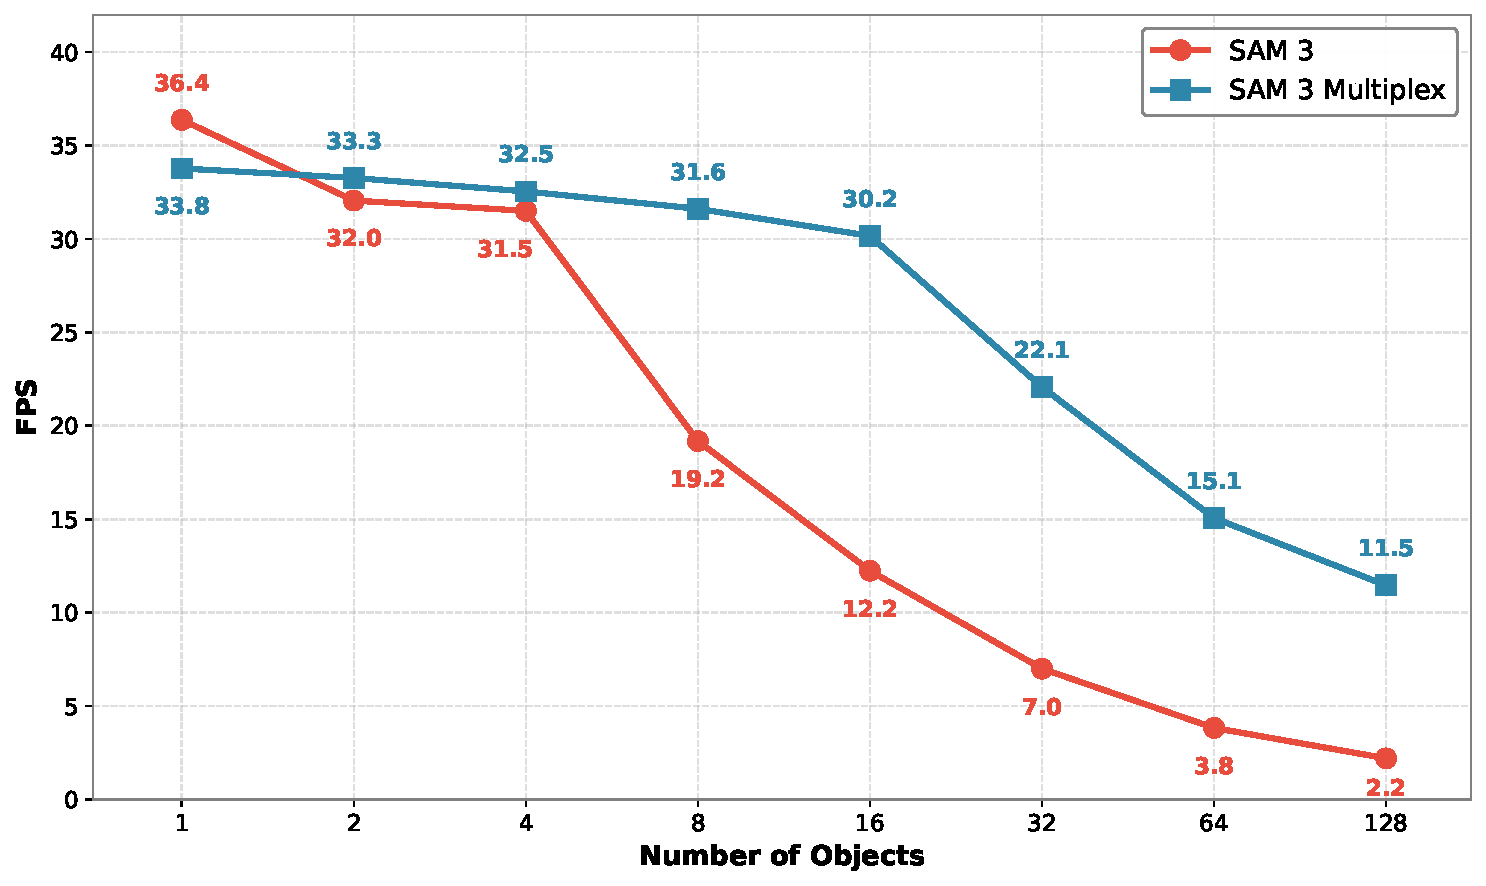
\includegraphics[width=0.6\linewidth]
    {figures/h_multiplex/multiplex_efficiency.pdf}
    \vspace{-5pt}
	\caption{FPS comparison of \model vs. \model Multiplex across varying object counts on a single H100 GPU.} 
	\label{fig:multiplex_efficiency}
    \vspace{-10pt}
\end{figure}



